\documentclass[12pt]{article}

%Allgemeine Einstellungen

%Abstände
\usepackage[a4paper,left=3cm,right=3cm,top=3cm,bottom=3.5cm,headsep=12pt]{geometry}%Bottom extra 0.5cm für Footer

%Deutsches Sprachpacket
\usepackage[german,ngerman]{babel}

%Times New Roman
\usepackage{mathptmx}

%Titelseite einbinden
\usepackage{pdfpages}

%1.5-Zeilenabstand
\usepackage[onehalfspacing]{setspace}

%Stil der Überschriften, siehe ueberschriften.sty
\usepackage[numeric]{ueberschriften}

%Stil des Inhaltsverzeichnisses, siehe inhaltsverzeichnis.sty
\usepackage[numeric]{inhaltsverzeichnis}

%Abkürzungsverzeichnis, siehe abk_verzeichnis.sty
\usepackage{abk_verzeichnis}

%Stil der Fußzeilen, siehe fusszeilen.sty
\usepackage{fusszeilen}

%Literaturverzeichnis und Zitate, siehe literatur.sty
\usepackage{literatur}

%Stil für Header und Footer, siehe header_footer.sty
%Wenn nicht erwünscht, müssen auch die Befehle \frontmatter, \mainmatter auskommentiert werden
\usepackage{header_footer}

%Stile für Code-Ausschnitte, siehe codes.sty
\usepackage{codes}

%Stile für Anhänge, Bilder, ...
\usepackage{anhang}

%Silbentrennung (manche Worte werden am Zeilenende nicht getrennt, diese müssen dann nachgetragen werden)
\usepackage[T1]{fontenc}
\hyphenation{öf-fent-lich-en}

%DEBUGGING (Zeigt Boxen an)
%\usepackage{showframe}
\setlength{\skip\footins}{12pt}

%Für Zeilenumbrüche in Tabellenzellen
\usepackage{makecell}
%Falls Tabellen oder Bilder komisch in den Text fließen
\usepackage{placeins}

%Ab hier kommt spezifisches für dieses Dokument
\definecolor{grayBack}{rgb}{0.8,0.8,0.8}

\begin{document}

\renewcommand{\mytitle}{Dokumentation/Tutorial}%Titel für oben links
\renewcommand{\myauthor}{Dr. Frank N. Furter}%Name für unten links

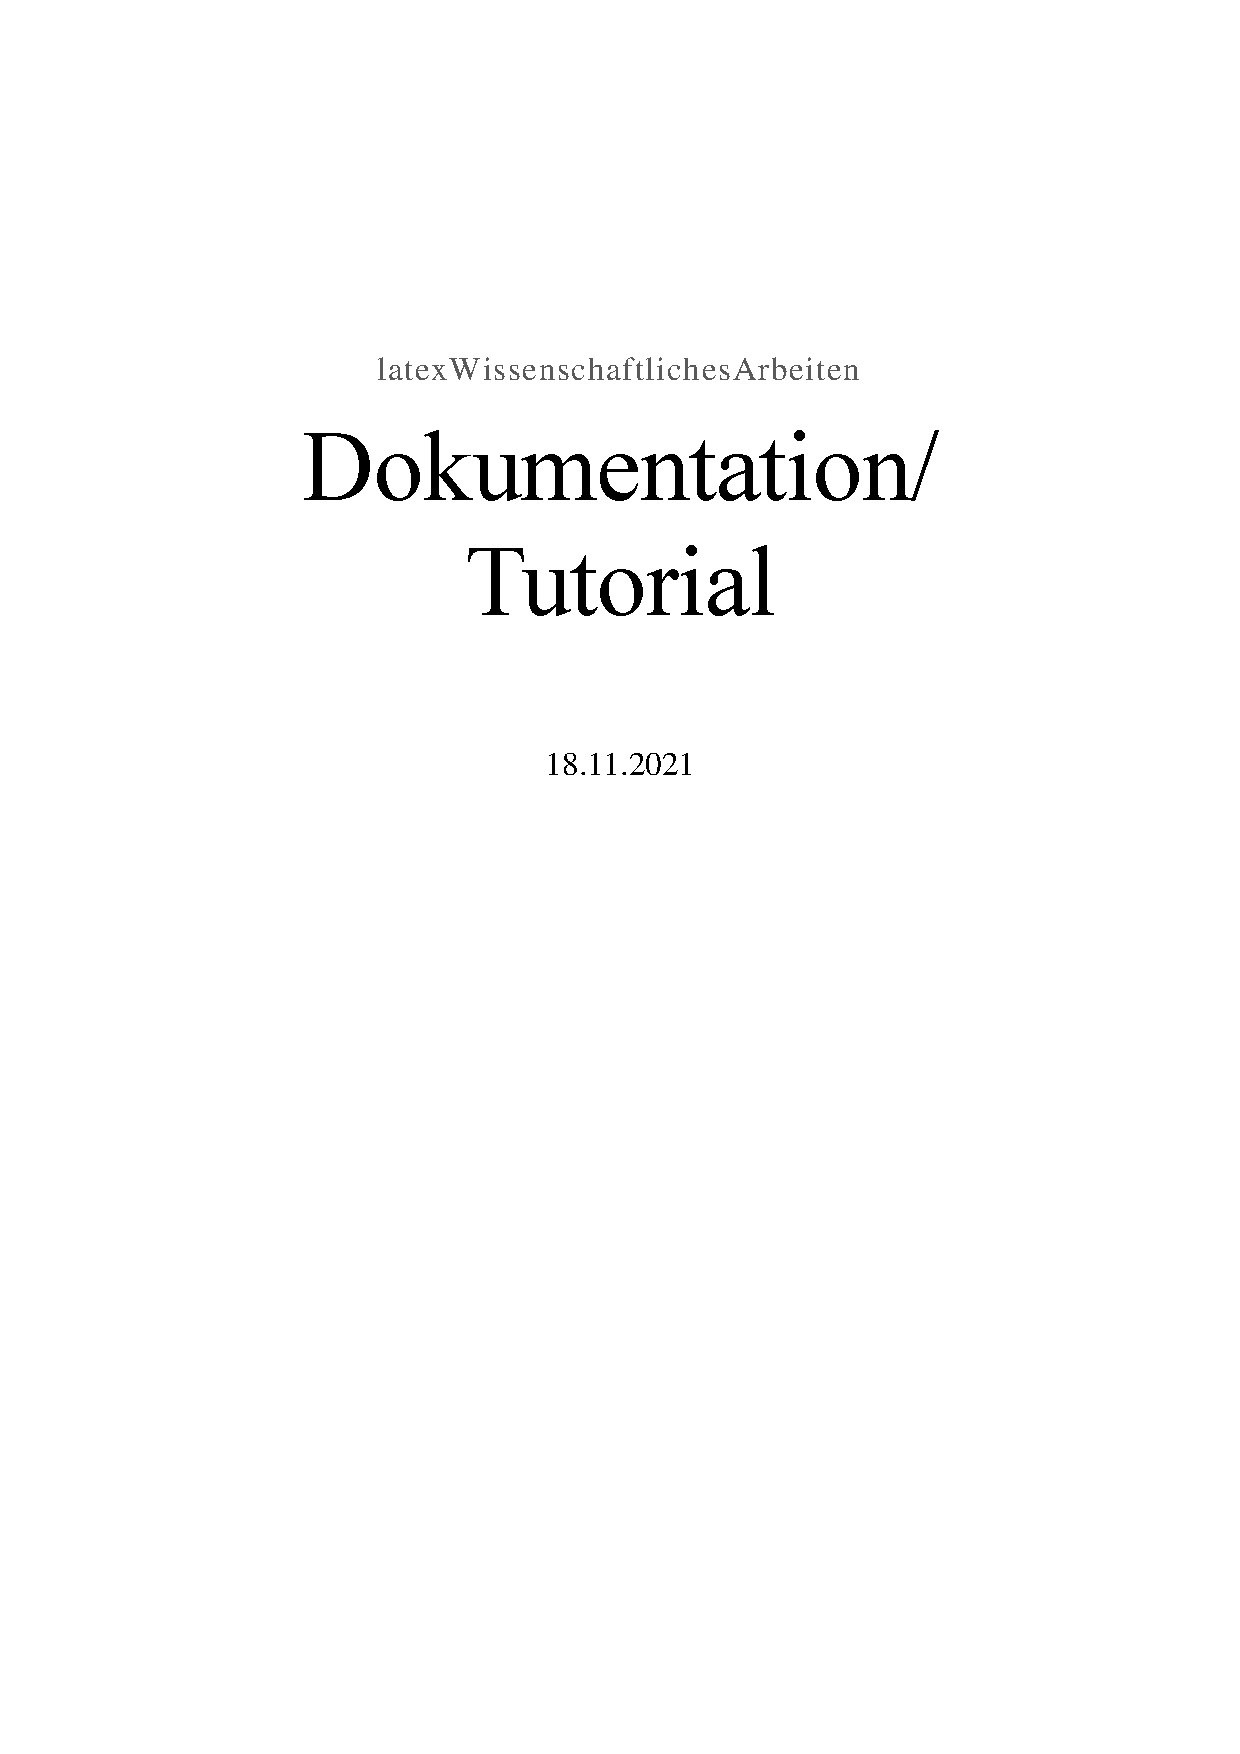
\includepdf[pages={1-}]{titelseiteAlternative.pdf}

\frontmatter%Stil des Headers/Footers ändern

\pagenumbering{Roman}

\addcontentsline{toc}{part}{Abkürzungsverzeichnis}%Abk-Verz. ins Inhaltsverzeichnis
\printabbreviations%abk_verzeichnis.sty
\clearpage
\renewcommand{\plaintitle}{Abbildungsverzeichnis}
\addcontentsline{toc}{part}{Abbildungsverzeichnis}
{\def\makebox[#1][#2]#3{#3}%
\listoffigures
}
\clearpage
\renewcommand{\plaintitle}{Tabellenverzeichnis}
\addcontentsline{toc}{part}{Tabellenverzeichnis}
{\def\makebox[#1][#2]#3{#3}%
\listoftables
}
\clearpage
\renewcommand{\plaintitle}{Inhaltsverzeichnis}%Titel für oben Rechts
%Defbox, damit gepunktete Linie bis zur Zahl geht
{\def\makebox[#1][#2]#3{#3}%
	\tableofcontents
}

\addtocontents{toc}{\vspace{24pt}}%Freiraum im ToC

\clearpage
\mainmatter%Stil des Headers/Footers ändern
\pagenumbering{arabic}

\part{Tutorial}
In dieser Doku wird der Aufbau und die Funktionsweise dieser Vorlage und der dahinter stehenden Mechanismen erläutert. Ein grundlegendes Verständnis von \textit{LaTeX} wird vorausgesetzt. Diese Doku wurde mithilfe der Vorlage erstellt.
\section{Dokumentenstruktur}
Die Struktur kann bis zu sechs Kapitelebenen umfassen und basiert auf der Dokumentenklasse \textit{article}. Die Nummerierung kann in numerischer Form erfolgen:\\\textit{\textbackslash usepackage[numeric]\{ueberschriften\}}\\[6pt]
\colorbox{grayBack}{\begin{minipage}{\textwidth}
\vspace{5pt}
\hspace{5pt}1\hspace{15pt}Part\\
\-\hspace{25pt} 1.1\hspace{10pt}Section\\
\-\hspace{50pt} 1.1.1\hspace{5pt}Subsection\\
\-\hspace{80pt} 1.1.1.1\hspace{5pt}Subsubsection\\
\-\hspace{120pt} 1.1.1.1.1\hspace{5pt}Paragraph\\
\-\hspace{170pt} 1.1.1.1.1.1\hspace{5pt}Subparagraph\vspace{5pt}
\end{minipage}
}\\[6pt]
Oder in alpha-numerlischer Form:\\\textit{\textbackslash usepackage[latour]\{ueberschriften\}}\\[6pt]
\colorbox{grayBack}{\begin{minipage}{\textwidth}
\vspace{5pt}
\hspace{5pt}A\hspace{10pt}Part\\
\-\hspace{25pt} I\hspace{10pt}Section\\
\-\hspace{45pt} 1\hspace{10pt}Subsection\\
\-\hspace{65pt} a)\hspace{10pt}Subsubsection\\
\-\hspace{85pt} aa)\hspace{5pt}Paragraph\\
\-\hspace{105pt} (1)\hspace{10pt}Subparagraph\vspace{5pt}
\end{minipage}
}

\section{Abkürzungsverzeichnis}
Die abkürzungen werden aus der Datei \textit{abkuerzungen.csv} bezogen. Dort können Sie einfach im CSV-Format eingetragen werden:\\[6pt]
\colorbox{grayBack}{\begin{minipage}{4cm}
\vspace{5pt}
\hspace{5pt}abk;bed\\
\-\hspace{5pt}z.B.;zum Beispiel\\
\-\hspace{5pt}s.o.;siehe oben\vspace{5pt}
\end{minipage}
}\\[6pt]
\textbf{Achtung:} Die erste Zeile muss so stehen bleiben!

\section{Literaturverzeichnis und Zitate}
Für LaTeX gibt es ein eigenes Tool zum Management von Literatur und Zitaten, \textit{BibLaTeX}. Allerdings sind individuelle Anpassungen dort sehr kompliziert. Deshalb wird hier eine eigene Lösung verwendet.
\subsection{Workflow}
Hier werden der Ablauf dieser eigenen Lösung und die groben technischen Abläufe beschrieben.
\subsubsection{Web-GUI}
Die Konfiguration der Literatur-Typen und -Einträge findet auf einer kleinen Webanwendung statt, welche in diesem Projekt mitgeliefert wird. Rufe dazu in einer Kommandozeile in deinem lokalen Projektordner \textit{WA\_ LaTeX.exe} auf. Dieser Befehl startet einen lokalen Webserver auf Port 8081. Nun kannst du in deinem Browser \textit{http://localhost:8081/overview} aufrufen:
\begin{center}
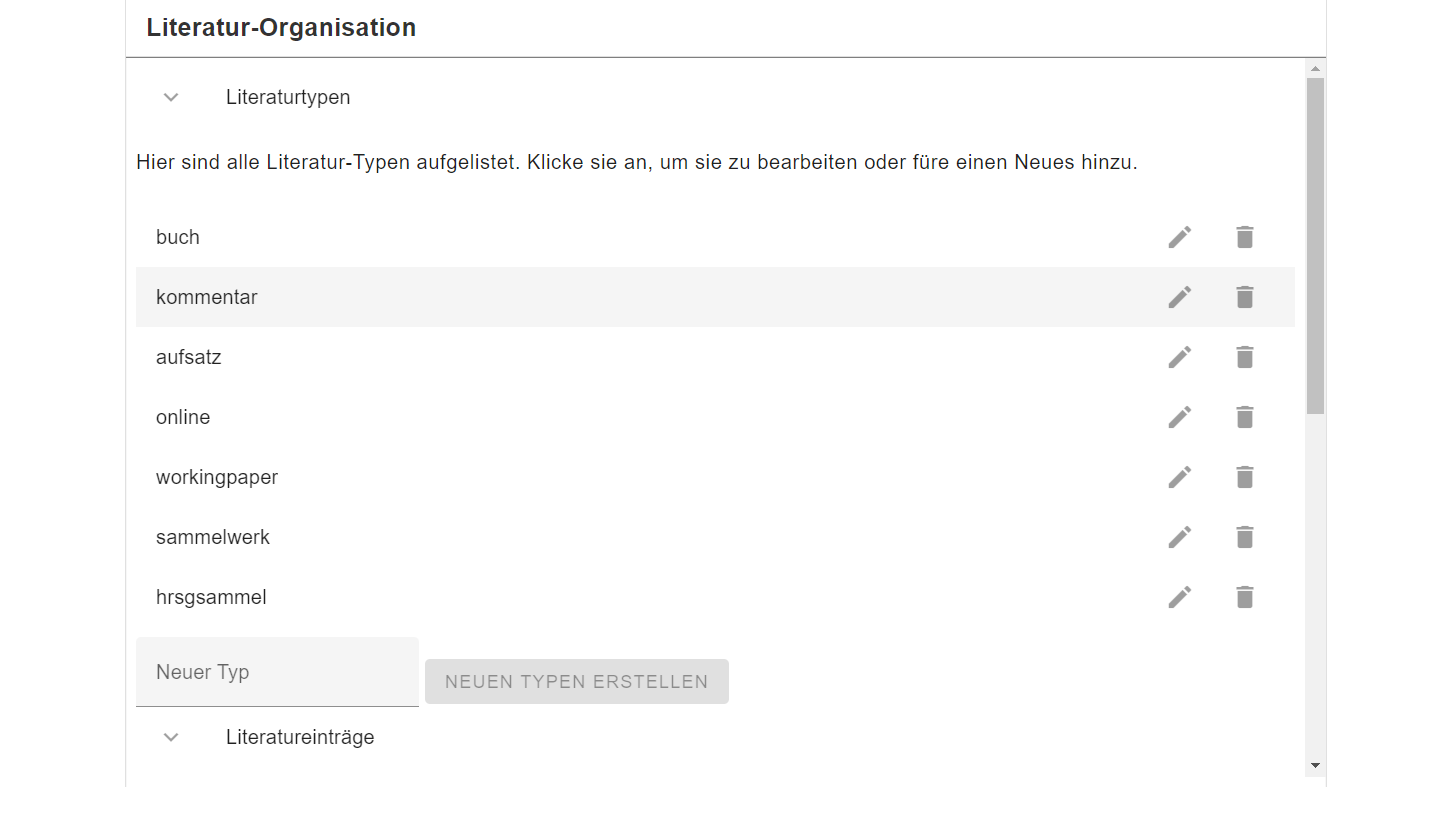
\includegraphics[width=\textwidth]{dokuImages/gui1.png}
\end{center}
Hier können zunächst Literaturtypen bearbeitet, gelöscht oder erstellt werden.
\begin{center}
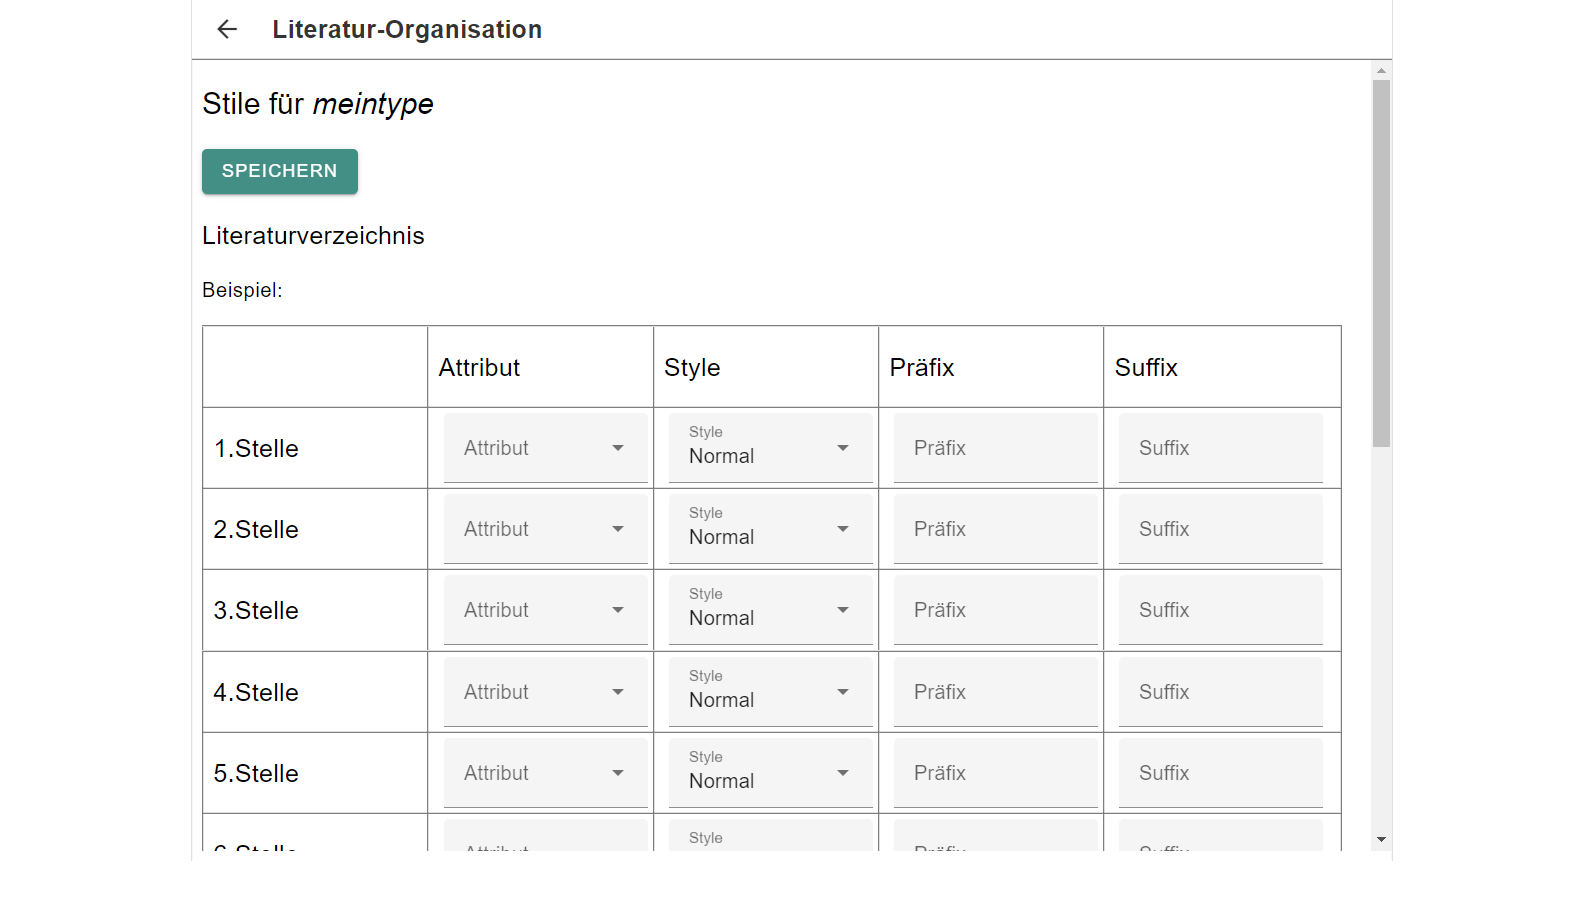
\includegraphics[width=\textwidth]{dokuImages/gui_2.png}
\end{center}
Es können jeweils die im Literaturverzeichnis und in Zitaten gewünschten Attribute ausgewählt und nach Wunsch mit einem Style (normal, kursiv, fett) und einem Prefix/Suffix versehen werden. Wie das Ergebnis aussehen würde, ist am Beispiel zu sehen:
\begin{center}
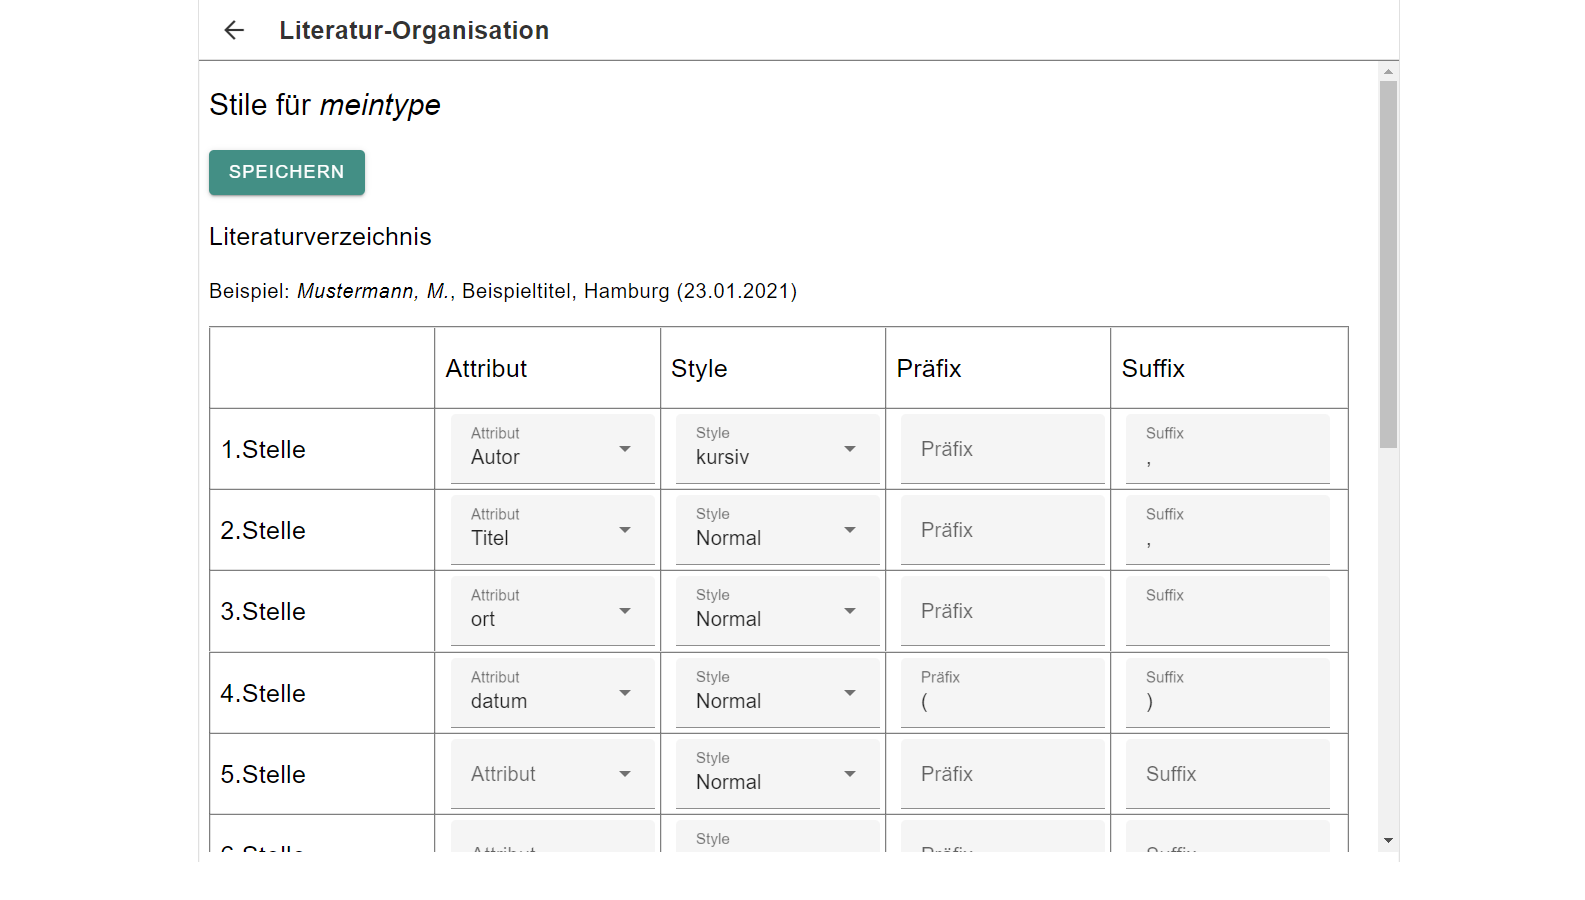
\includegraphics[width=\textwidth]{dokuImages/gui_21.png}
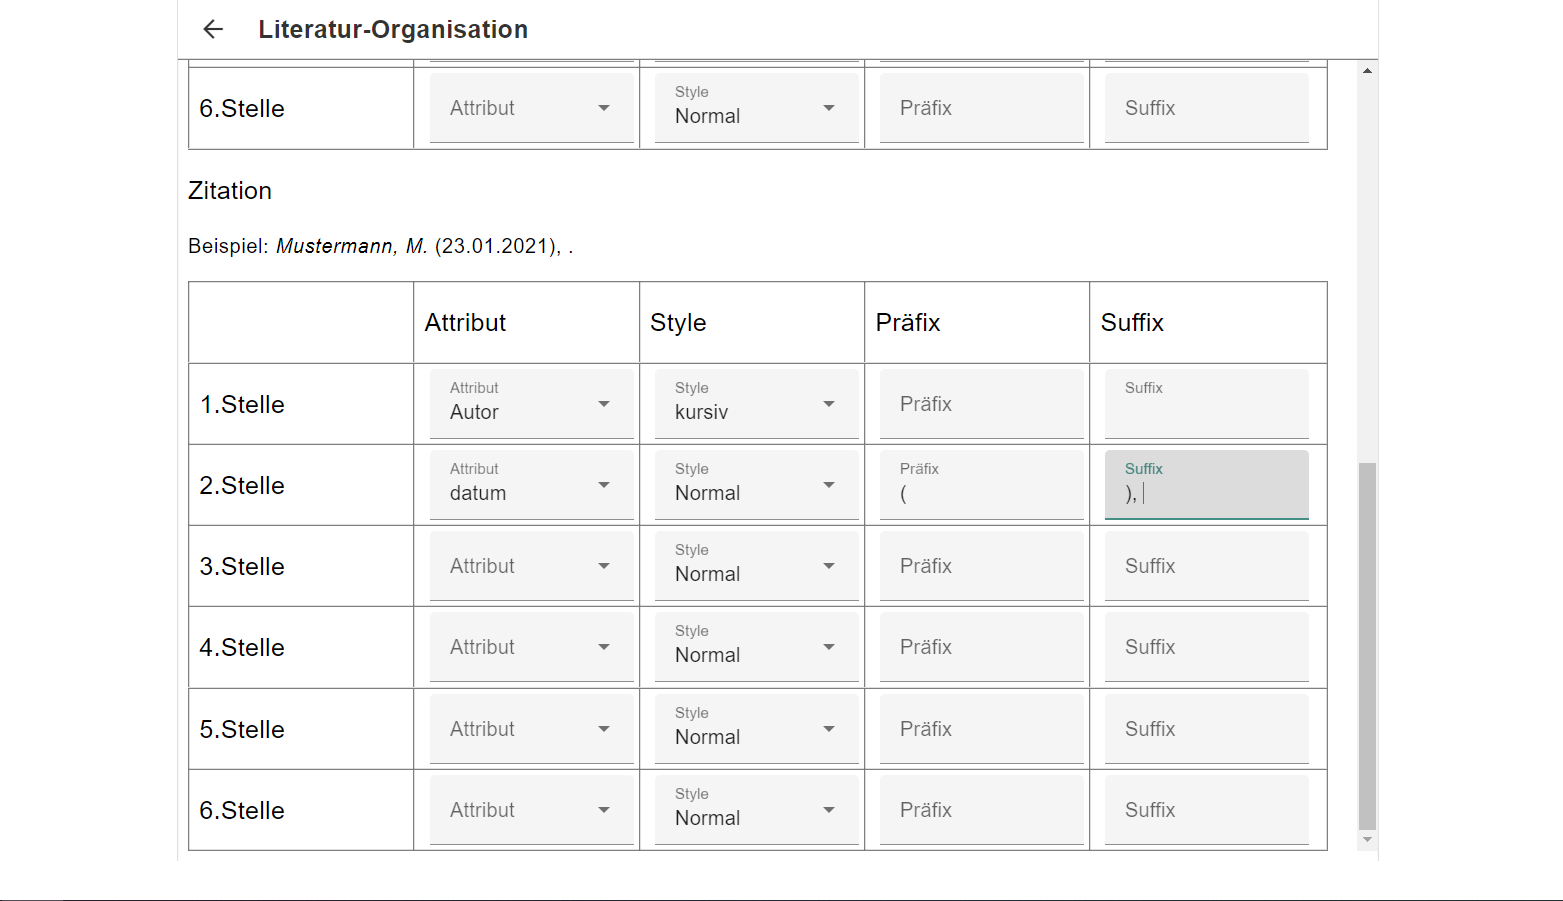
\includegraphics[width=\textwidth]{dokuImages/gui41.png}
\end{center}
Im nächsten Schritt können Einträge dieses Typen hinzugefügt werden:
\begin{center}
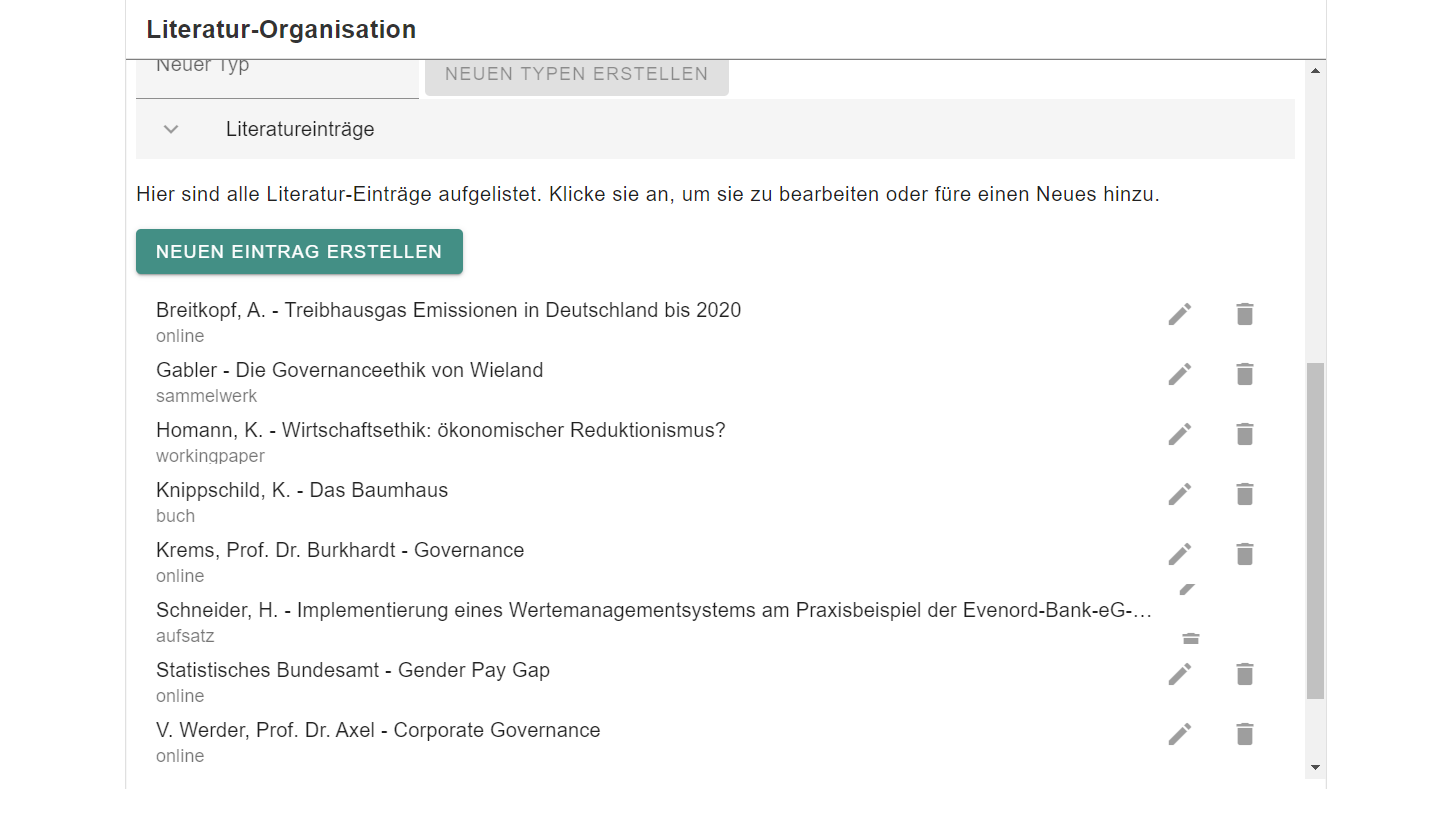
\includegraphics[width=\textwidth]{dokuImages/gui2.png}
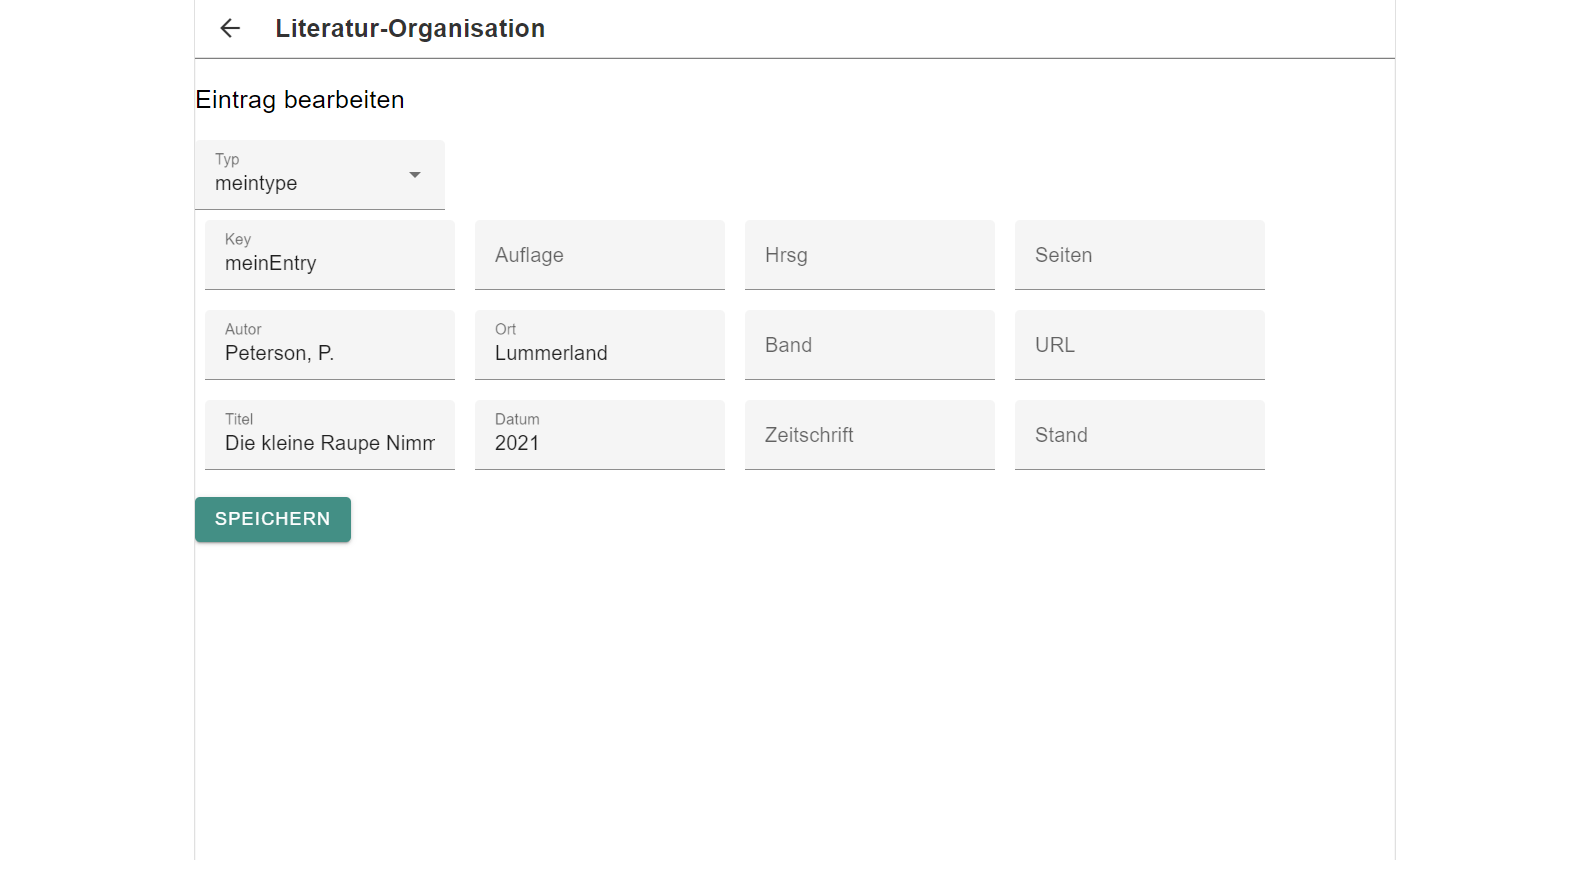
\includegraphics[width=\textwidth]{dokuImages/gui_4.png}
\end{center}
Wenn nun das LaTeX-Dokument erneut kompiliert wird, tuacht im Literaturverzeichnis der neue Eintrag auf:
\begin{center}
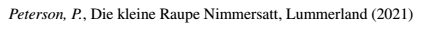
\includegraphics[width=\textwidth]{dokuImages/litentry.png}
\end{center}
Zitate können über den Befehl \textit{\textbackslash citebib\{KEY\}\{SEITE\}\{LEER oder Vgl. \}} gemacht werden.\citebib{meinEntry}{S.15}{Vgl. }

\section{Tabellen- und Abbildungsverzeichnis}
Um Tabellen darzustellen kann das \textit{table}-Envirmonment verwendet werden. Um eine Verschiebung zu vermeiden, können vor und nach der Tabelle \textit{\textbackslash FloatBarrier} verwendet werden:
\FloatBarrier
\begin{table}[!ht]
\begin{tabular}{|p{3cm}|l|l|}
Zelle 1.1 & 1.2 & 1.3\\
\end{tabular}
\end{table}
\FloatBarrier

\section{Häufig auftretende Fehler/Warnungen}

\clearpage
\frontmatter%Stil des Headers/Footers ändern
\renewcommand{\plaintitle}{Literaturverzeichnis}
\pagenumbering{Roman}
\setcounter{page}{5}
\addtocontents{toc}{\vspace{24pt}}
\addcontentsline{toc}{part}{Literaturverzeichnis}%Literatur-Verz. ins Inhaltsverzeichnis
\printMyBibliography

\end{document}